\documentclass[10pt]{beamer}
\usetheme{Warsaw}
\usepackage[T1]{fontenc}
\usepackage[utf8]{inputenc}
\usepackage{chronosys}
\usepackage{graphicx}
\usepackage{multicol} 
\usepackage{hyperref}

\begin{document}

\begin{frame}
\frametitle{KINETIC AND BUILDING LOD2}
\begin{figure}

    \begin{minipage}{0.33\textwidth}
        \centering
        
\includegraphics[width=0.6\textwidth]{../image/logo_irma.png}
    \end{minipage}%
    \begin{minipage}{0.33\textwidth}
        \centering
        
\includegraphics[width=0.6\textwidth]{../image/logo-numpex-web-2.png}
    \end{minipage}%
    \begin{minipage}{0.33\textwidth}
        \centering
        
\includegraphics[width=0.6\textwidth]{../image/logo-ufr-mathinfo-unistra-1.jpg}
    \end{minipage}
    
    \vspace{0.5cm} 
    
   
    \begin{minipage}{0.33\textwidth}
        \centering
        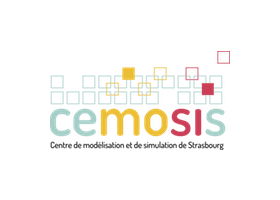
\includegraphics[width=0.6\textwidth]{../image/logoCemosis-square-e1469167314407.png}
    \end{minipage}%
    \begin{minipage}{0.33\textwidth}
        \centering
        
\includegraphics[width=0.6\textwidth]{../image/HiDALGO2-logo.jpg}
    \end{minipage}%
    \begin{minipage}{0.33\textwidth}
        \centering
        
\includegraphics[width=0.6\textwidth]{../image/logo-inria-.jpg}
    \end{minipage}
    
\end{figure}

\vspace{0.5cm} 

Intern: Demuth Axel \\
Supervisor: Vincent Chabannes, Pierre Alliez, Florent Lafarge

\end{frame}

\begin{frame}
    \frametitle{Table of Contents}
    \begin{multicols}{2} % Diviser la page en deux colonnes
        \tableofcontents
    \end{multicols}
    \end{frame}


\section{Introduction}
\begin{frame}{Introduction}
  \begin{itemize}
    \item Need of more sophisticated tool for energy simulations
    \item As a part of Exa-MA project from Numpex : CEMOSIS want to port Ktirio application to exascale power 
    \item My objectives was to developed a geometric reconstruction tools of buillding using Kinetic algorithm
  \end{itemize}

\end{frame}


\subsection{Context}
\begin{frame}{Context}
\begin{figure}
    \begin{minipage}{0.45\textwidth}
    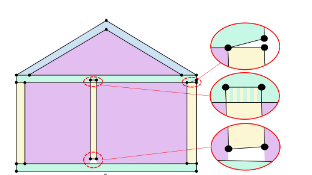
\includegraphics[width=0.9\textwidth]{../image/mesh_with_issue.png}
    \caption{Mesh with issues}
    
\end{minipage}
    \begin{minipage}{0.45\textwidth}
    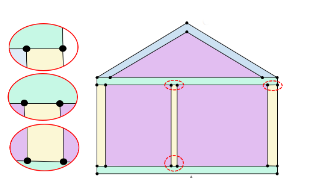
\includegraphics[width=0.9\textwidth]{../image/mesh_fixed.png}
    \caption{Mesh without issues}
\end{minipage}
\end{figure}
\end{frame}

\subsection{Issue with Kinetic Algorithm}
\begin{frame}{Issue with orientation}
    \begin{figure}
        \centering
        \begin{minipage}[b]{0.3\textwidth}
          \centering
          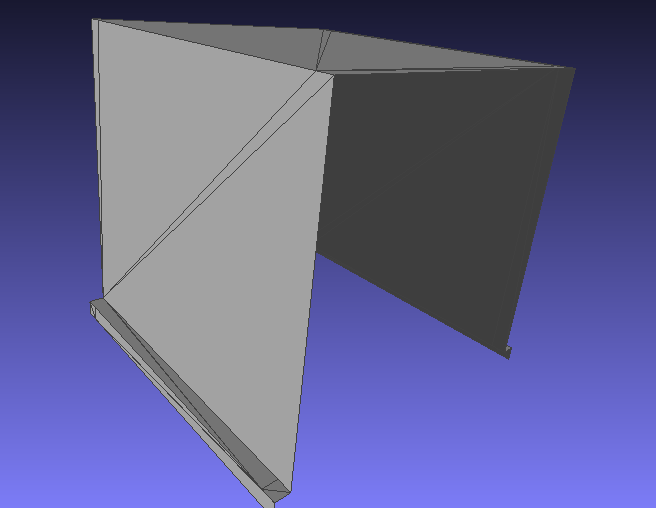
\includegraphics[width=\textwidth]{../image/cube_3faces.png}
          \caption{Cube not oriented}
        \end{minipage}%
        \begin{minipage}[b]{0.3\textwidth}
          \centering
          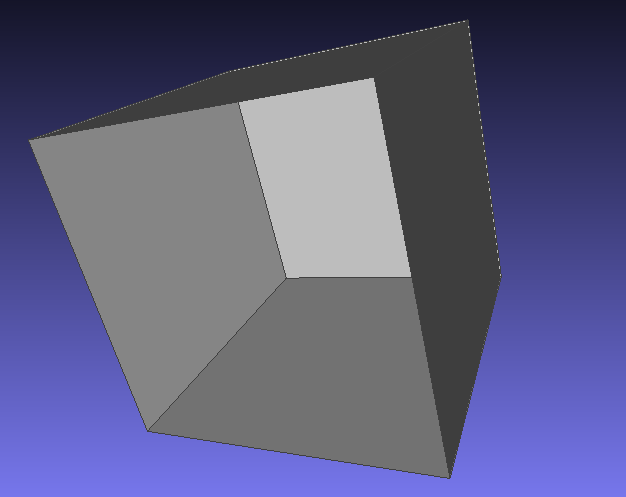
\includegraphics[width=\textwidth]{../image/cube_5faces.png}
          \caption{Cube badly oriented}
        \end{minipage}%
        \begin{minipage}[b]{0.3\textwidth}
          \centering
          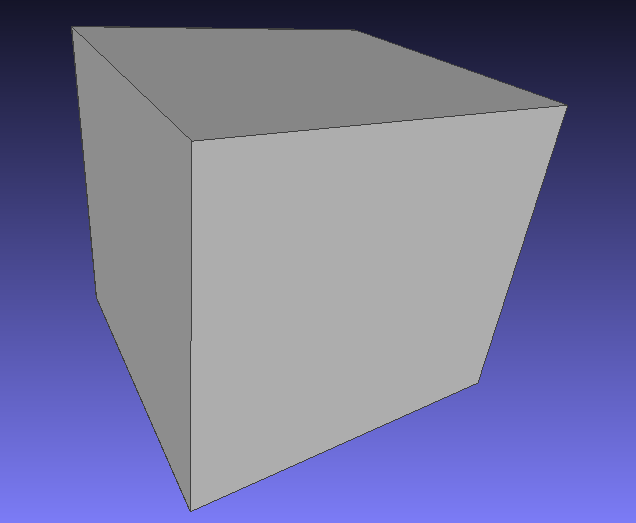
\includegraphics[width=\textwidth]{../image/bon_cube.png}
          \caption{Cube oriented by CGAL}
        \end{minipage}
      \end{figure}
\end{frame}

\begin{frame}{Self Intersection issue}
    \begin{figure}
        \centering
        \begin{minipage}[b]{0.23\textwidth}
          \centering
          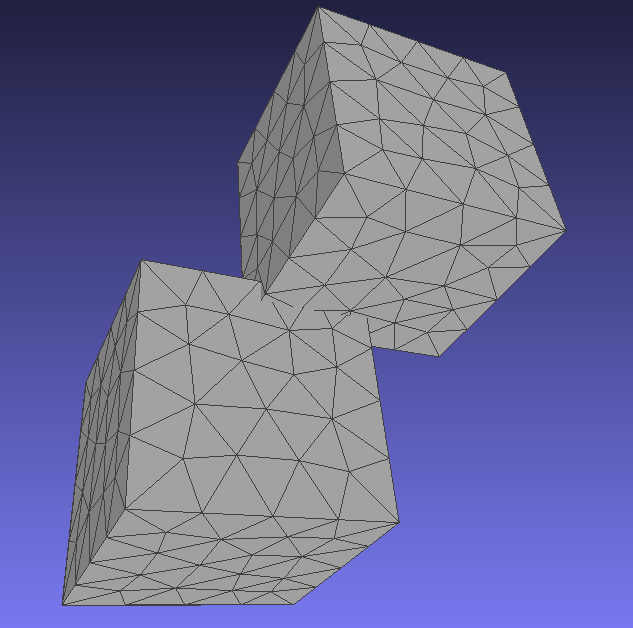
\includegraphics[width=\textwidth]{../image/2cubes.png}
          \caption{Two cube self intercting}
        \end{minipage}\hfill
        \begin{minipage}[b]{0.23\textwidth}
          \centering
          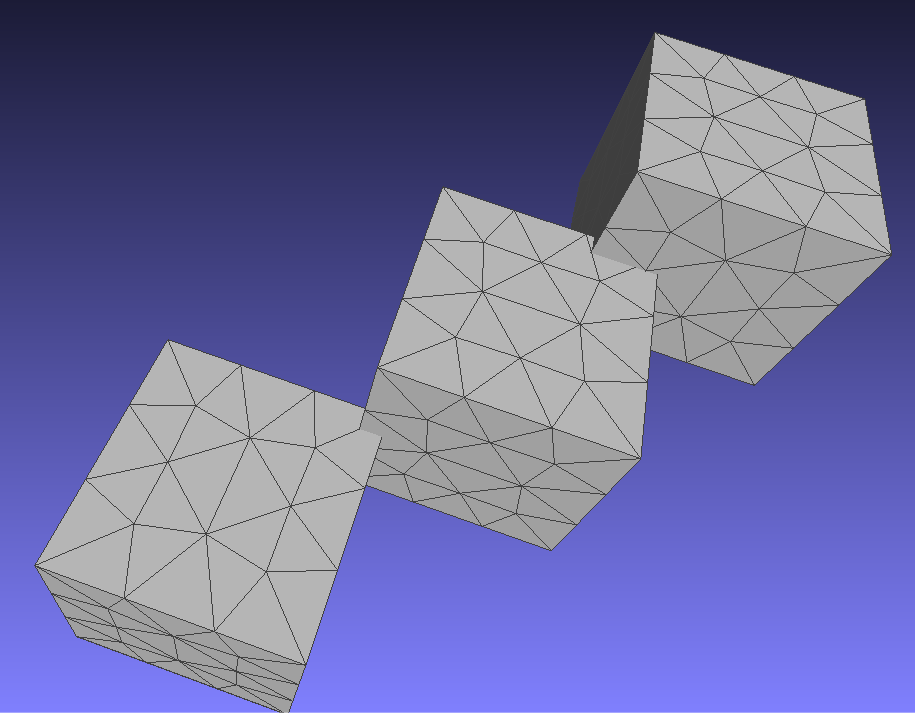
\includegraphics[width=\textwidth]{../image/3cubes.png}
          \caption{Two cubes intersecting a third one}
        \end{minipage}\hfill
        \begin{minipage}[b]{0.23\textwidth}
          \centering
          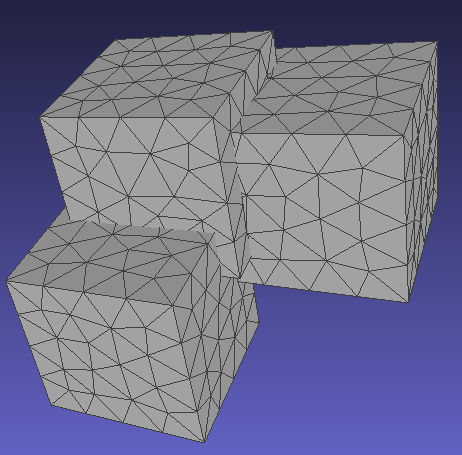
\includegraphics[width=\textwidth]{../image/3cubes_tresproche.png}
          \caption{Three cubes self intersecting}
        \end{minipage}\hfill
        \begin{minipage}[b]{0.23\textwidth}
          \centering
          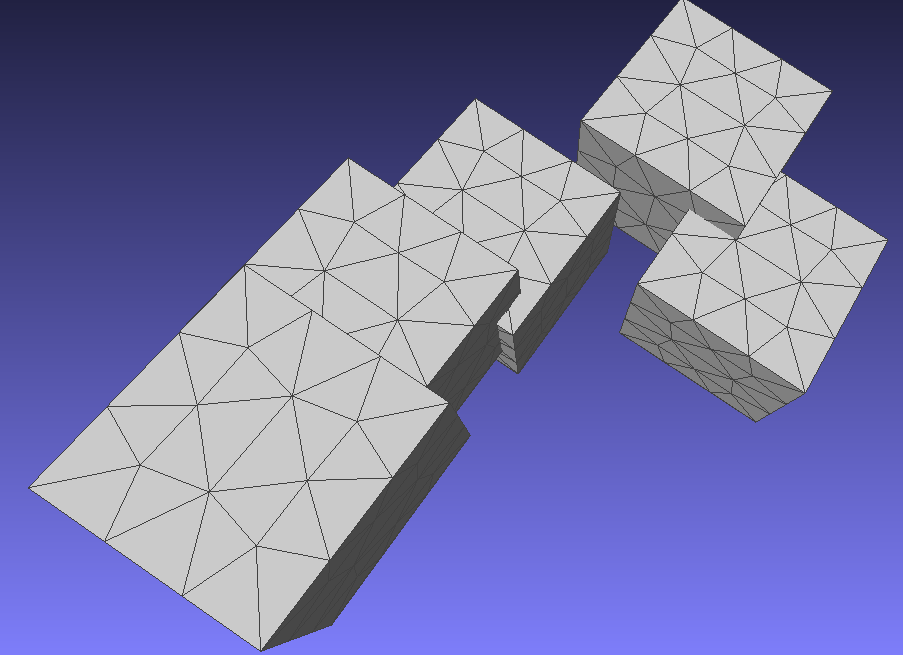
\includegraphics[width=\textwidth]{../image/5cubes.png}
          \caption{Five cubes  intercting randomly}
        \end{minipage}
      \end{figure}    
\end{frame}

\begin{frame}
\begin{figure}
    \centering
    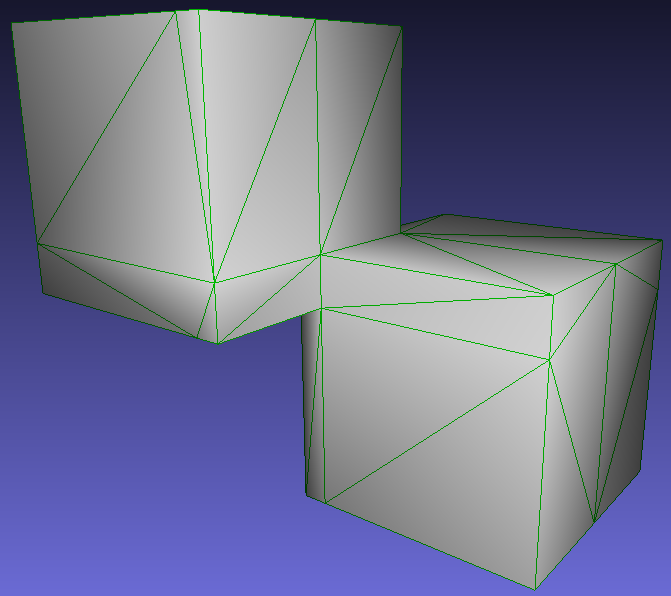
\includegraphics[width=0.4\textwidth]{../image/2_cubes_fixed.png}
    \caption{Two Cubes fixed}
  \end{figure}
All other result in a execution error
\end{frame}

\subsection{Objectives}
\begin{frame}{Objectives}
    \begin{itemize}
        \item Check the validity of the Mesh
        \item Create a workflow for automatic generation using KSR Algorithm
        \item Keep the correspondence of surfaces between both meshes
        \item Run some simulations using the Feel++ library
    \end{itemize}
\end{frame}

\subsection{CGAL}
\begin{frame}{CGAL}
    \begin{itemize}
        \item C++ library for geometric calculations, providing data structures for mesh generation and manipulation.
    \end{itemize}
    \vspace{0.5cm}
    The main packages utilized are:
    \begin{itemize}
        \item \texttt{CGAL::Polygon\_mesh\_processing}
        \item \texttt{CGAL::Surface\_mesh}
        \item \texttt{CGAL::Point\_set\_processing}
        \item \texttt{CGAL::IO\_streams}
        \item \texttt{CGAL::AABB\_tree}
    \end{itemize}
    
\end{frame}


\section{Data}
\subsection{Files Format}
\begin{frame}{File Format}
\begin{itemize}
    \item IFC : Standart for buillding data modeling,similar to class oriented code
    \item CityGML : 3D format for city modeling with representation of geographic details
    \item STL : 3D Modeling format 
    \item OBJ :A standard file format for 3D models
    \item OFF :  A file format for 3D mesh data
    \item PLY :  A file format for 3D mesh data,stocking the cloud point of the mesh 
    \item MSH : A file format for mesh data use by GMSH software
\end{itemize}
\end{frame}

\subsection{Software and Data}
\begin{frame}{Software}
    \begin{itemize}
        \item Github : Platforme for collaborating work on a project
        \item Visual Studio Code : Versatil tools for coding with various extensions
        \item Paraview : Open-source data analysis and visualisation
        \item Meshlab : A tool for processing,editing,visualisation of 3D mesh
        \item GMSH : a 3D finite element mesh generator
    \end{itemize}

\end{frame}

\begin{frame}{Data}
    The following Data were given by Vincent Chabannes
    \begin{figure}
        \begin{minipage}{0.33\textwidth}
            \centering
            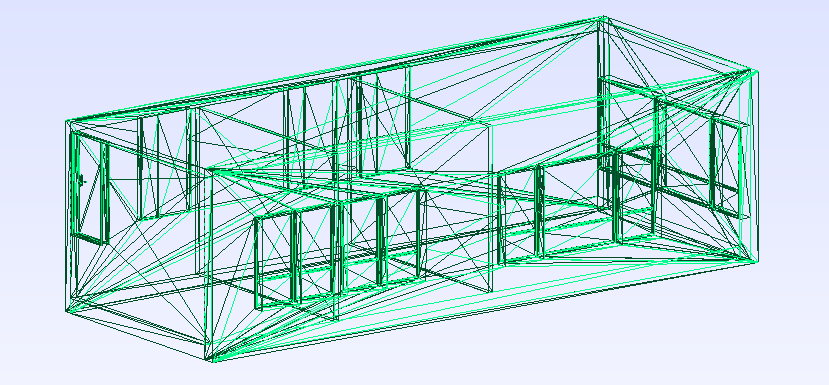
\includegraphics[width=0.9\textwidth]{../image/3zones_stl.png}
        \end{minipage}%
        \begin{minipage}{0.33\textwidth}
            \centering
            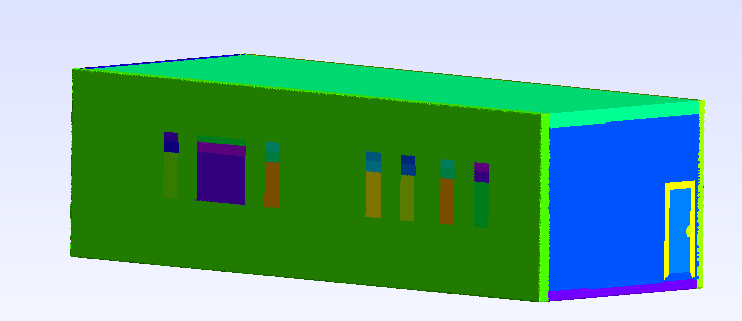
\includegraphics[width=0.9\textwidth]{../image/label_three_zone.png}
        \end{minipage}
        \caption{Three zones mesh}
    \end{figure}
    \begin{figure}
        \begin{minipage}{0.33\textwidth}
            \centering
            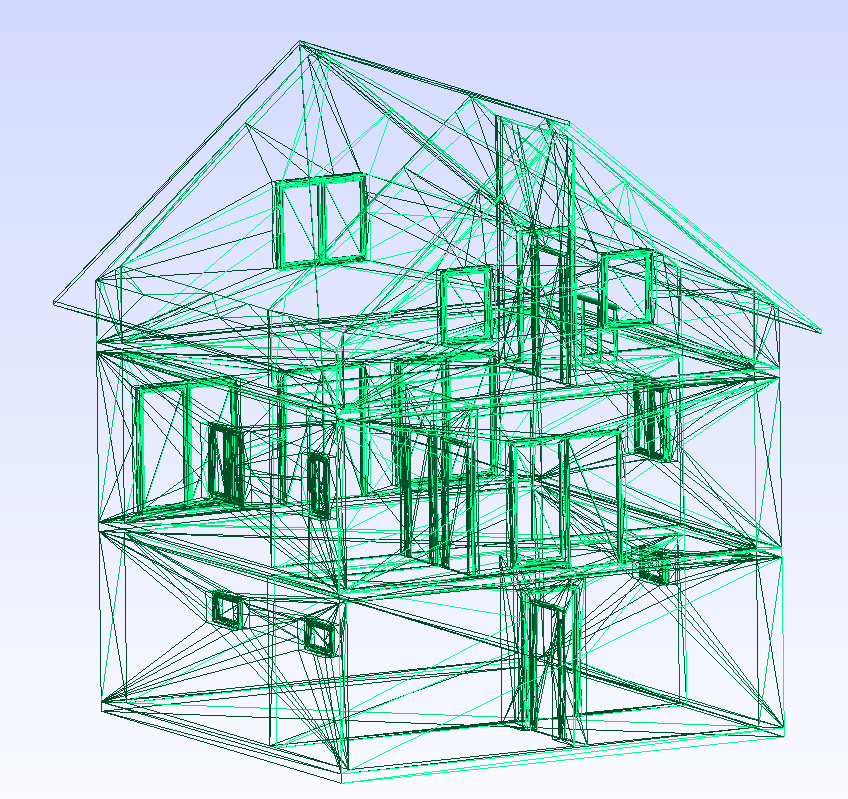
\includegraphics[width=0.9\textwidth]{../image/jasmin_stl.png}
        \end{minipage}
        \begin{minipage}{0.33\textwidth}
            \centering
            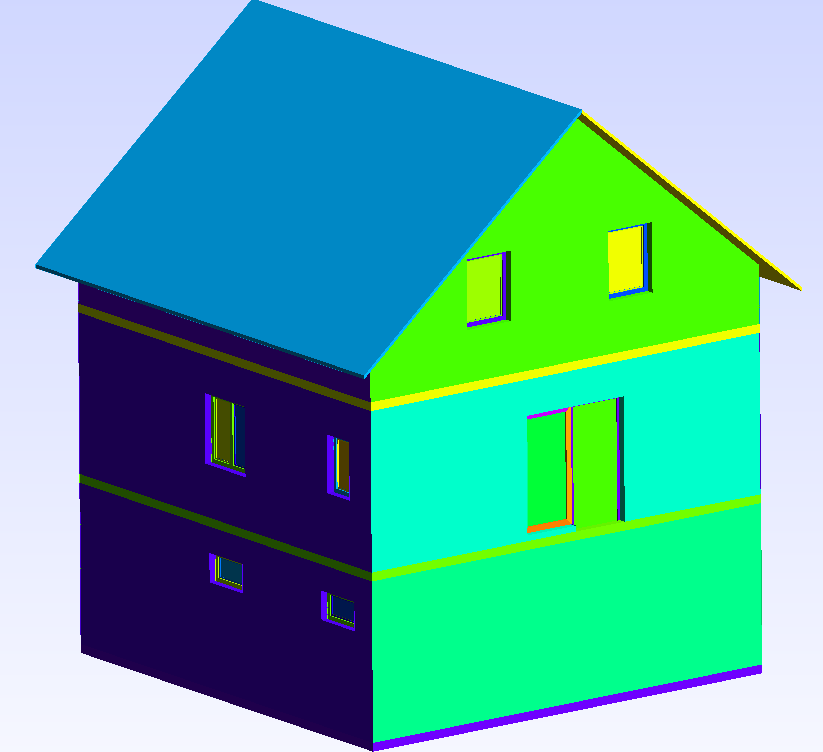
\includegraphics[width=0.9\textwidth]{../image/ACJasmin_1.png}
        \end{minipage}
        \caption{ACJasmin mesh}
    \end{figure}
\end{frame}


\section{Methodology}
\subsection{Kinetic}
\begin{frame}{Kinetic}
We get information from a INRIA report \cite{yu:hal-03767910}
Kinetic algorithm is an geometric algorithm generate 3D mesh from a point clouds,it uses  geometric primitive with an energy based model to fit the primitives to the model.

Energy formule: 
\newline
\begin{center}
    $        U(x) = w_f U_f(x) + w_s U_s(x) + w_c U_c(x)       $
\end{center}

to calculate the best primitive to fit the mesh.
then we have a list of geometric operation on each primitive
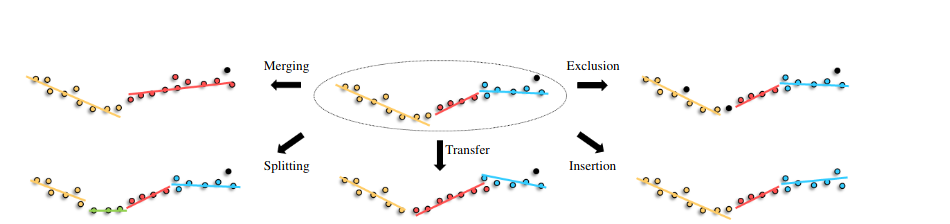
\includegraphics[scale=0.35]{../image/primitives_operation.png}
\end{frame}

\subsection{preprocessing}
\begin{frame}{preprocessing}  
    To improve Kinetic outcome we pre-process the mesh :
    \begin{itemize}
        \item Isotropic remeshing of the mesh
        \item Unified and regularize the mesh with grid simplify
        \item Fix self Intersection 
        \item Calcul normals
    \end{itemize}
\end{frame}

\subsection{Labelling}
\begin{frame}{Labelling}
    \textbf{Issue}: Inria developed a method to preserve the semantic information of IFC elements, but it has not yet been implemented in CGAL.

     Two potential solutions:
    \begin{itemize}
        \item Modify the Kinetic Solver to recognize and utilize markers on each point used to form a shape.
        \item Compare the input and output meshes to apply the same markers to the closest faces.
    \end{itemize}
\end{frame}

\begin{frame}{Labelling}
    Exemple of result of second solutions:
    \begin{figure}
        \centering
        \begin{minipage}{0.5\textwidth}
            \centering
            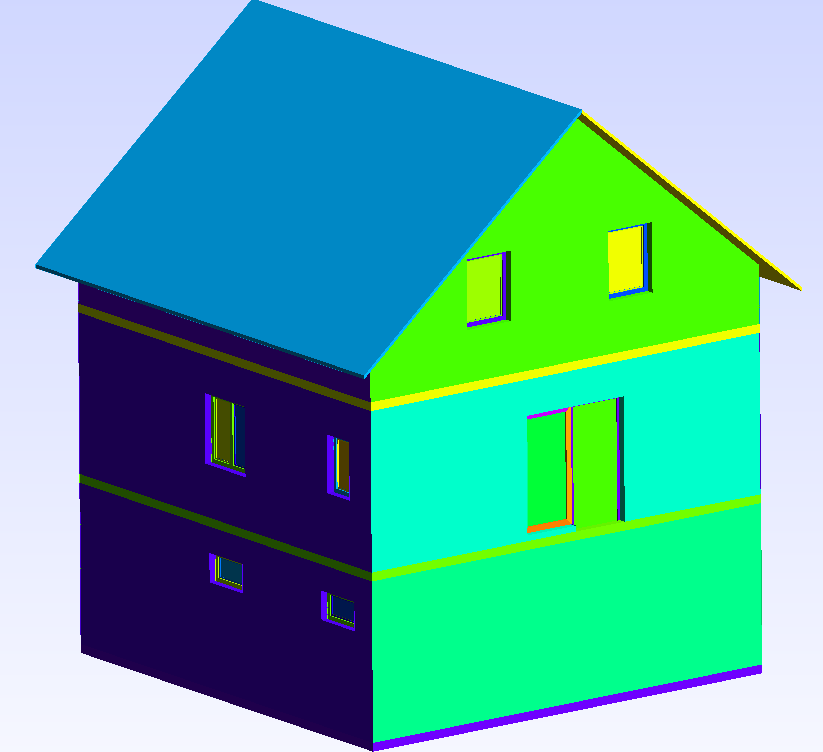
\includegraphics[width=0.9\textwidth]{../image/ACJasmin_1.png}
            \caption{Input Mesh}
            \label{fig:input_mesh}
        \end{minipage}%
        \begin{minipage}{0.5\textwidth}
            \centering
            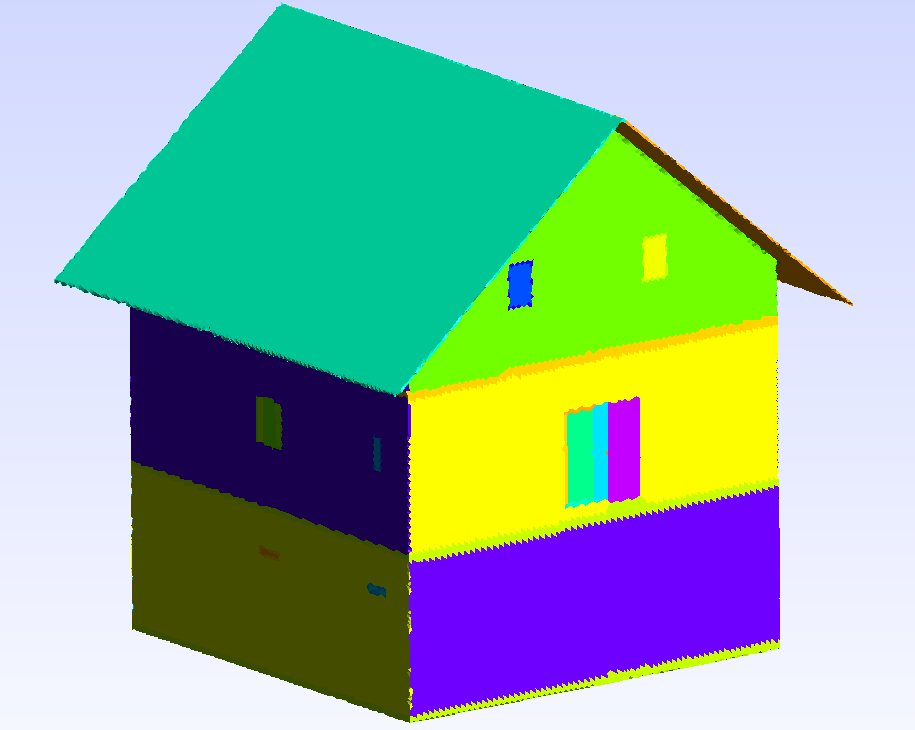
\includegraphics[width=1.05\textwidth]{../image/ACjasmin_label.png}
            \caption{Output Mesh}
            \label{fig:output_mesh}
        \end{minipage}
    \end{figure}
\end{frame}

\subsection{Metric}
\begin{frame}{Metric}
We also want to add method to check the quality off the output mesh
\begin{itemize}
    \item Properties Check (closed,connected,triangulated...)
    \item Correspondance between input and output
\end{itemize}
To check the Correspondance between mesh, we can compare 
bounding box of each labelled elements.

\begin{table}[h]
    \centering
    \caption{Bounding Box value}
    \begin{tabular}{|c|c|c|}
        \hline
         \% of marker correct & Three Zones & ACJasmin \\
        \hline
        <5\% & 22/57 & 3/82 \\
        between 5 and 10 \% & 11/57 & 7/82 \\
        between 10 and 20 \% & 13/57  & 9/82 \\
        \hline
    \end{tabular}
\end{table}
\end{frame}

\begin{frame}
    
    \begin{figure}
    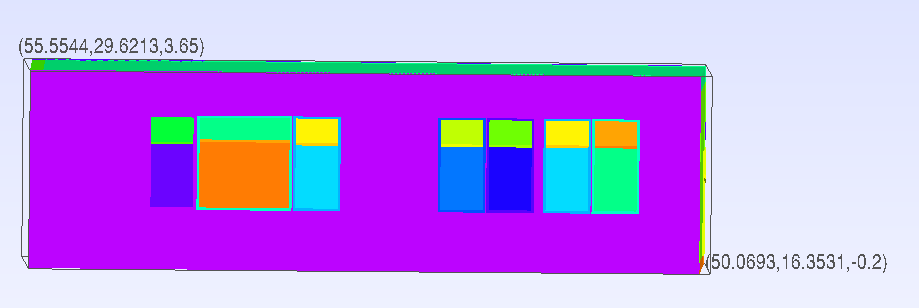
\includegraphics[width=0.9\textwidth]{../image/3_zones_input_bounding_box.png}
    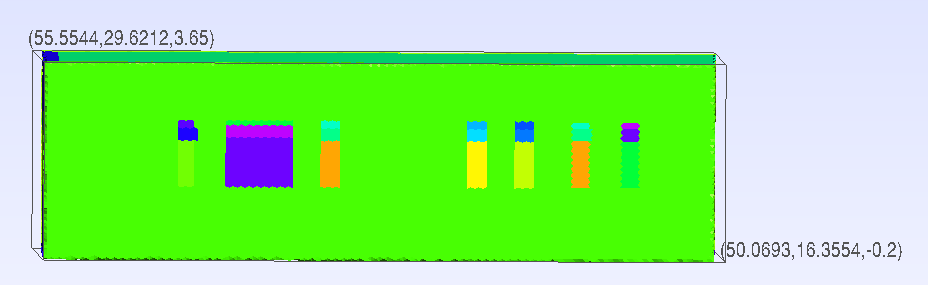
\includegraphics[width=0.9\textwidth]{../image/3zone_output_bounding_box.png}
    \caption{Three zones Bounding Boxe comparaison}
    \end{figure}
    
\end{frame}

\begin{frame}
    
    \begin{figure}
    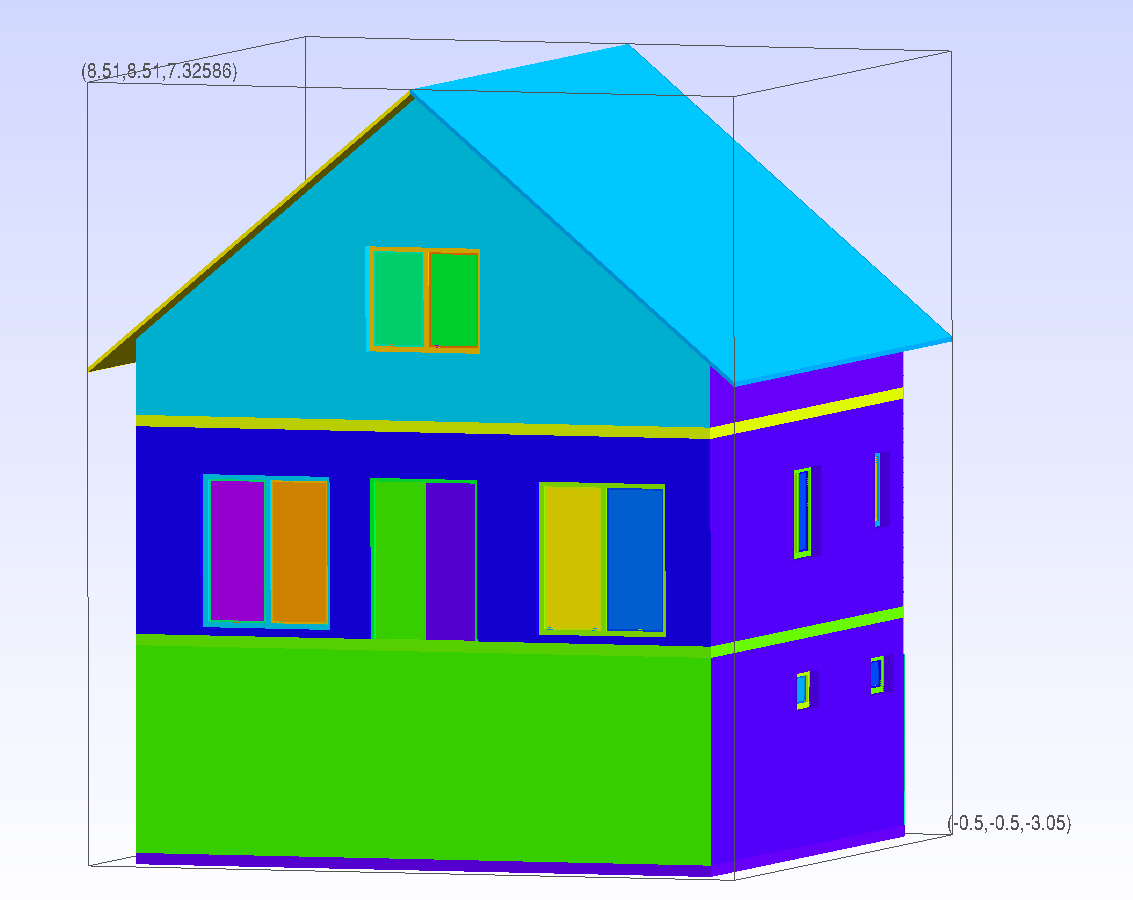
\includegraphics[width=0.4\textwidth]{../image/ACJasmin_input_bounding_box.png}
    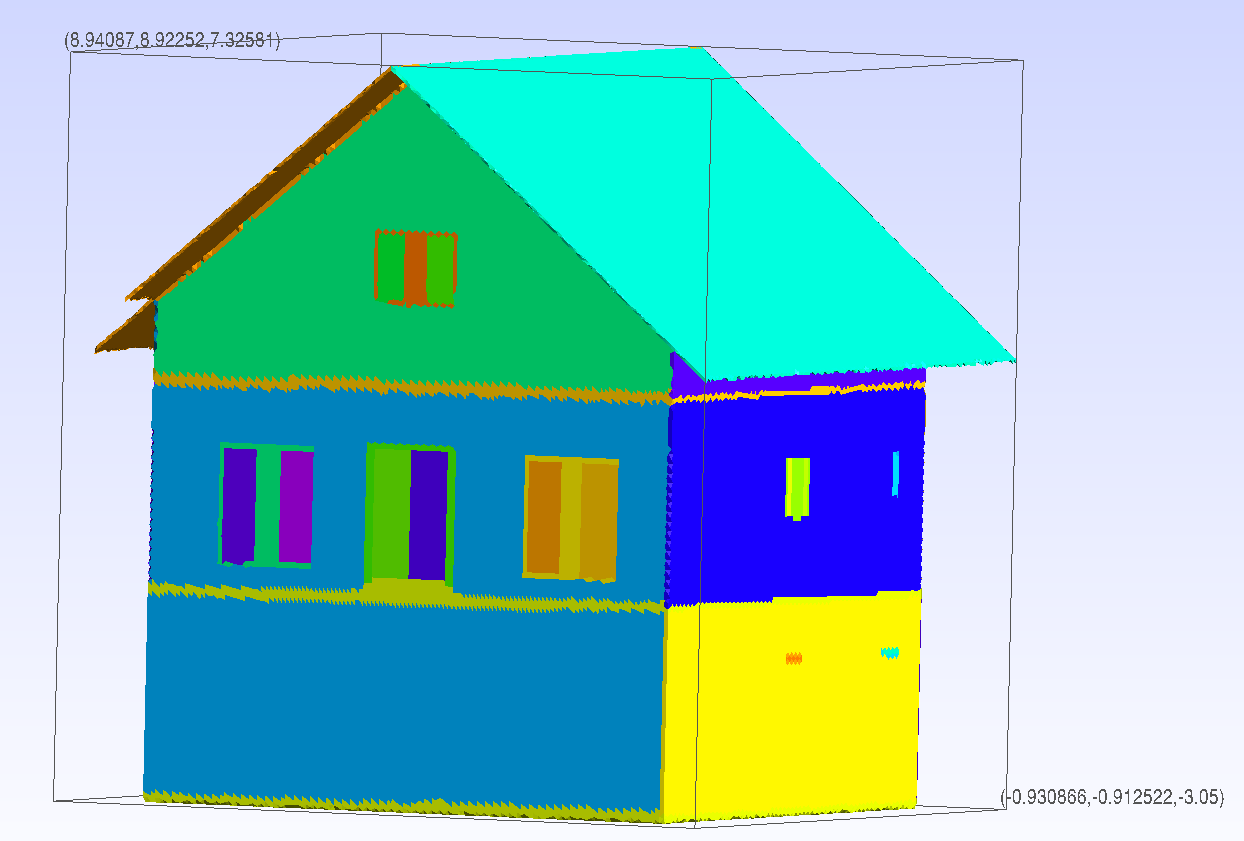
\includegraphics[width=0.47\textwidth]{../image/ACjasmin_output_bounding_box.png}
    \caption{ACJasmin Bounding Boxe comparaison}
    \end{figure}
    
\end{frame}

\section{Implementation}
\subsection{Contribution to Ktirio library}
\begin{frame}{}
  \begin{itemize}
    \item checkProperties{}
    \item gridSimplify{}
    \item remesh{}
    \item KSR{}
    \item IO function for off,ply,obj Files
    \item Point set class
    \item etc..
  \end{itemize}

\end{frame}

\subsection{test}
\begin{frame}{test}
    \begin{itemize}
        \item test on Surface Mesh Check
        \item test on Kinetic algorithm
        \item test on Point set class and manipulation function
    \end{itemize}
\end{frame}

\section{Result}
\subsection{Point cloud generation Result}
\begin{frame}{Point cloud}
    \begin{figure}
        \begin{minipage}{0.45\textwidth}
            \centering
            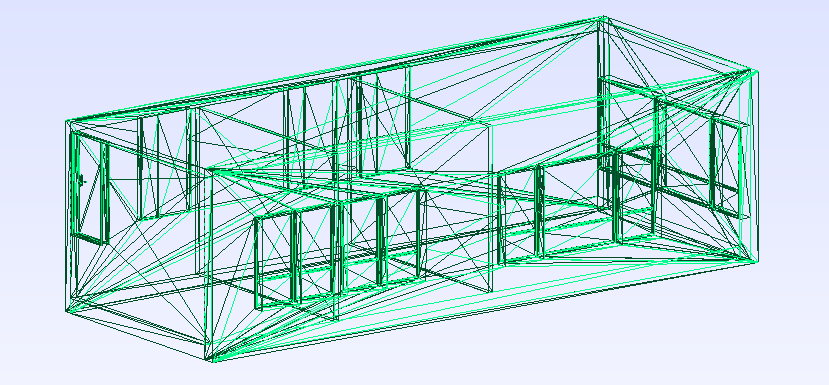
\includegraphics[width=0.9\textwidth]{../image/3zones_stl.png}
        \end{minipage}%
        \begin{minipage}{0.45\textwidth}
            \centering
            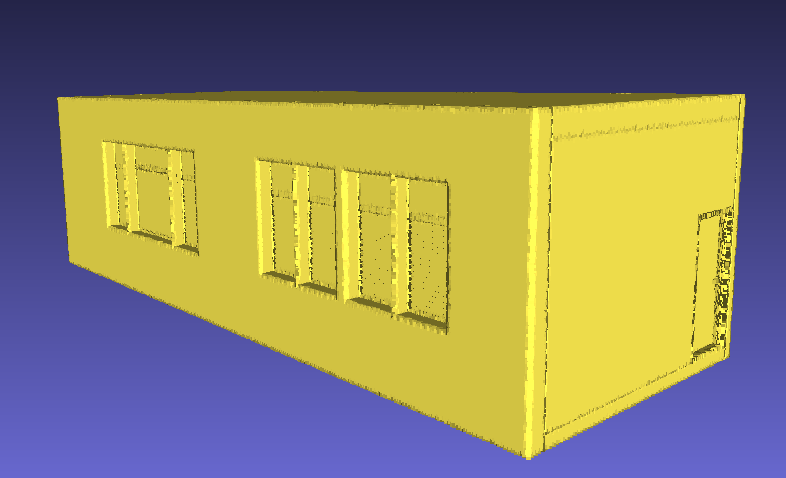
\includegraphics[width=0.9\textwidth]{../image/3zones_ply.png}
        \end{minipage}
        \caption{Three zones mesh point cloud}
    \end{figure}
\end{frame}

\begin{frame}
    \begin{figure}
        \begin{minipage}{0.45\textwidth}
            \centering
            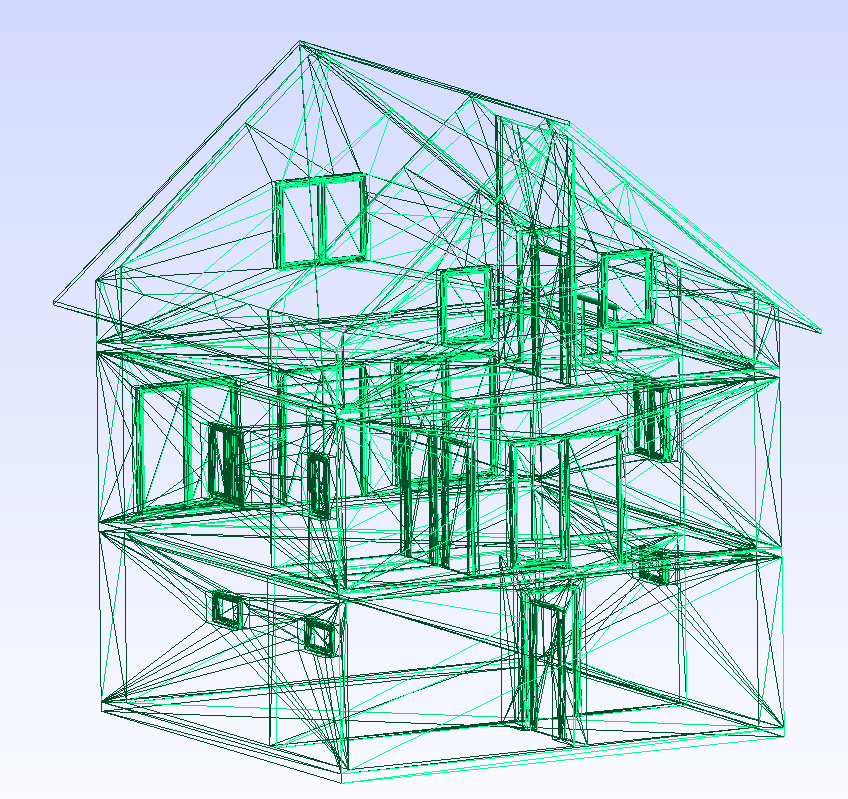
\includegraphics[width=0.9\textwidth]{../image/jasmin_stl.png}
        \end{minipage}
        \begin{minipage}{0.45\textwidth}
            \centering
            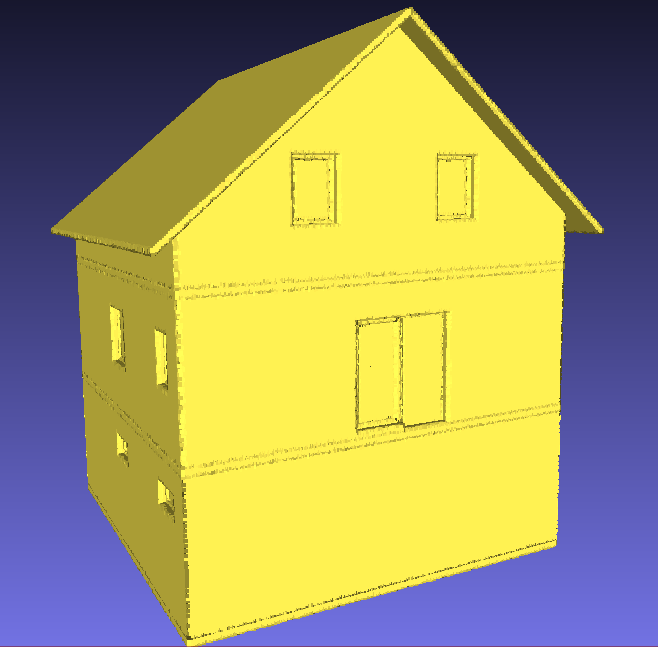
\includegraphics[width=0.9\textwidth]{../image/jasmin_ply.png}
        \end{minipage}
        \caption{ACJasmin mesh point cloud }
    \end{figure}
\end{frame}

\begin{frame}{Comparison of Kinetic Outcome}
    \begin{figure}
      \centering
      \begin{minipage}[b]{0.48\textwidth}
        \centering
        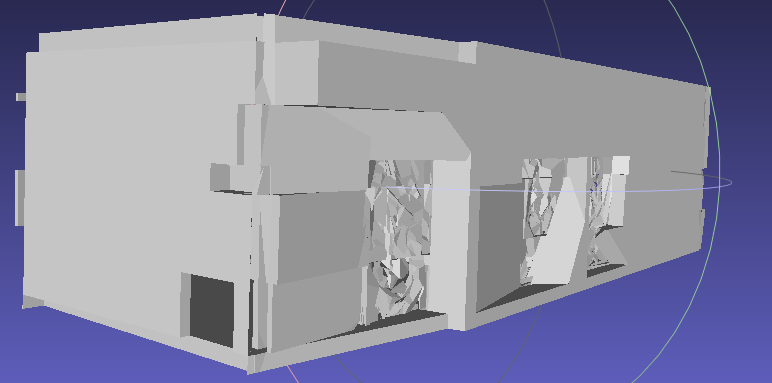
\includegraphics[width=\textwidth]{../image/3zones_v2_1.png}
        \caption{Old KSR outcome}
      \end{minipage}
      \hfill
      \begin{minipage}[b]{0.48\textwidth}
        \centering
        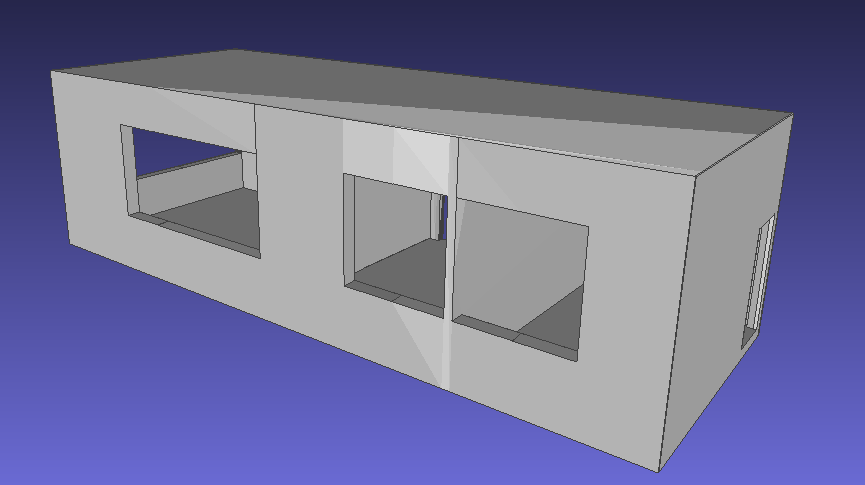
\includegraphics[width=\textwidth]{../image/3zones_final.png}
        \caption{New KSR outcome}
      \end{minipage}
    \end{figure}
\end{frame}

\begin{frame}{Comparison of 3 Zone Results}
\begin{figure}
  \centering
  \begin{minipage}[b]{0.48\textwidth}
    \centering
    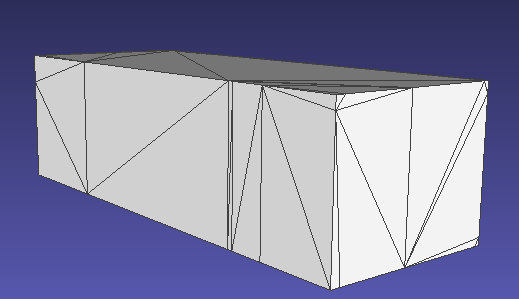
\includegraphics[width=\textwidth]{../image/3zone_500_0.06.png}
    \caption{3 Zone 500}
  \end{minipage}\hfill
  \begin{minipage}[b]{0.48\textwidth}
    \centering
    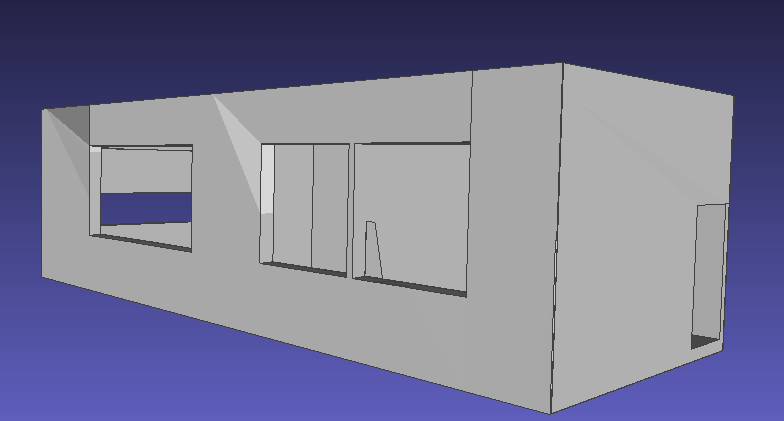
\includegraphics[width=\textwidth]{../image/3zones_45_0.06.png}
    \caption{3 Zones 45}
  \end{minipage}
\end{figure}
\end{frame}


\begin{frame}{Comparison of Jasmin Images}
    \begin{figure}
      \centering
      \begin{minipage}[b]{0.48\textwidth}
        \centering
        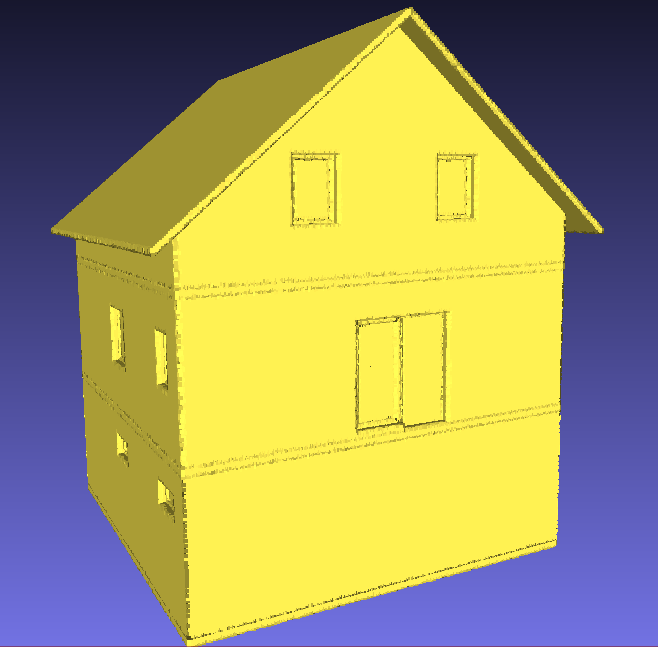
\includegraphics[width=\textwidth]{../image/jasmin_ply.png}
        \caption{Jasmin Ply}
      \end{minipage}\hfill
      \begin{minipage}[b]{0.48\textwidth}
        \centering
        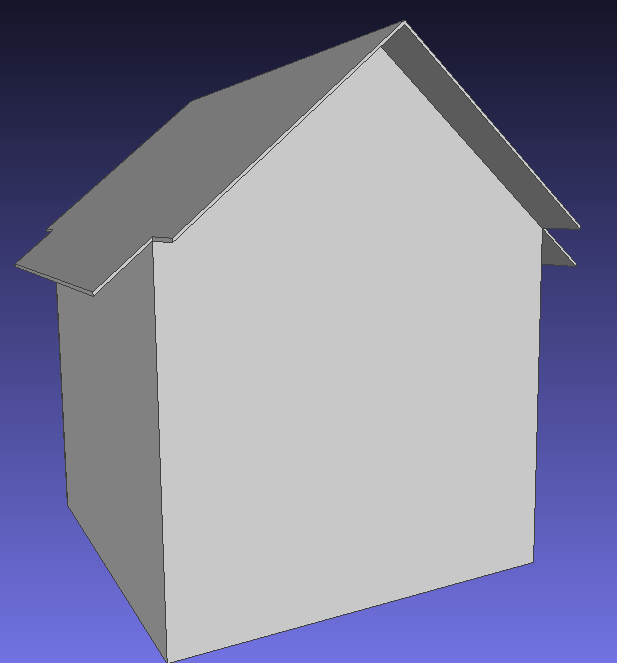
\includegraphics[width=\textwidth]{../image/jasmin.png}
        \caption{Jasmin Image}
      \end{minipage}
    \end{figure}
    \end{frame}

\subsection{Self Intersection Result}
\begin{frame}{Self Intersection fixing}
    \begin{figure}
        \centering
        \begin{minipage}[b]{0.23\textwidth}
          \centering
          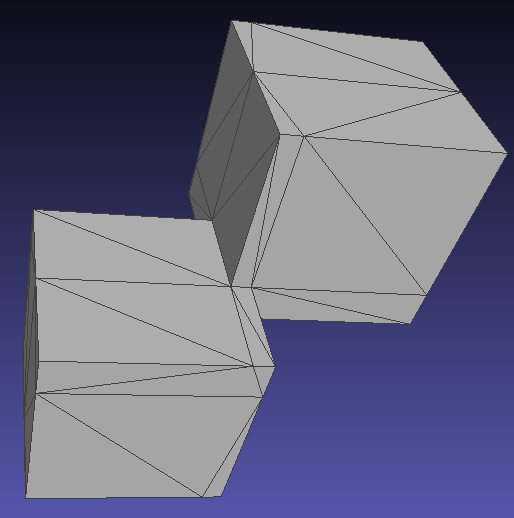
\includegraphics[width=\textwidth]{../image/2cubesksr.png}
          \caption{Same result as intro}
        \end{minipage}\hfill
        \begin{minipage}[b]{0.23\textwidth}
          \centering
          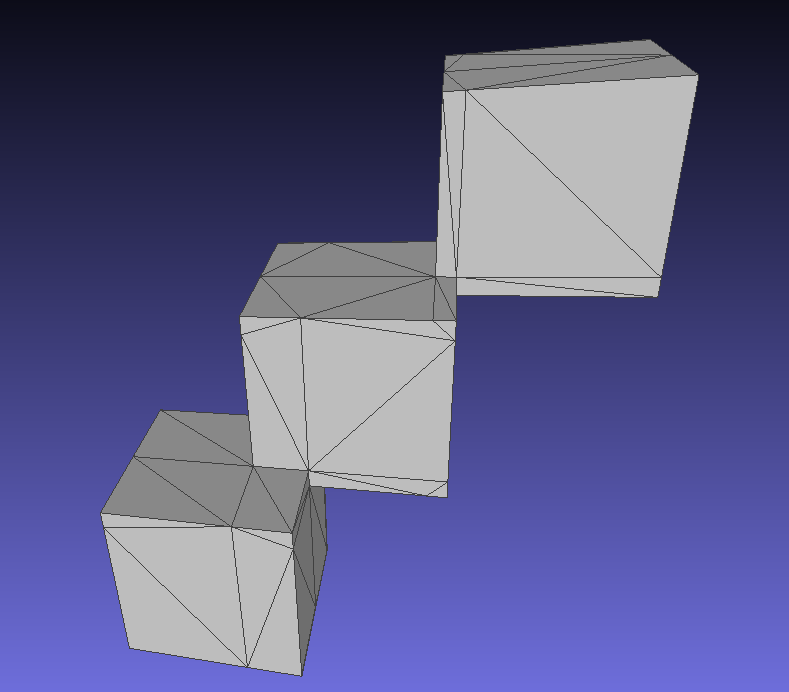
\includegraphics[width=\textwidth]{../image/3cubesksr2.png}
          \caption{Worked}
        \end{minipage}\hfill
        \begin{minipage}[b]{0.23\textwidth}
          \centering
          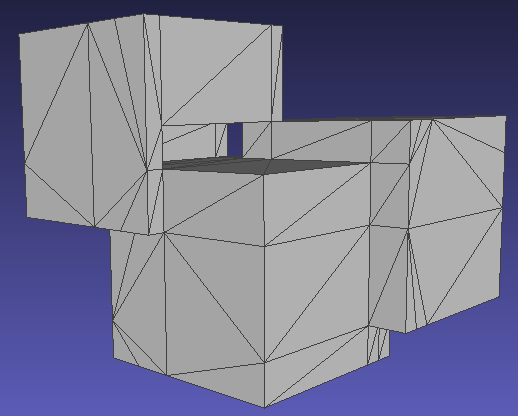
\includegraphics[width=\textwidth]{../image/3cubesksr.png}
          \caption{Worked}
        \end{minipage}\hfill
        \begin{minipage}[b]{0.23\textwidth}
          \centering
          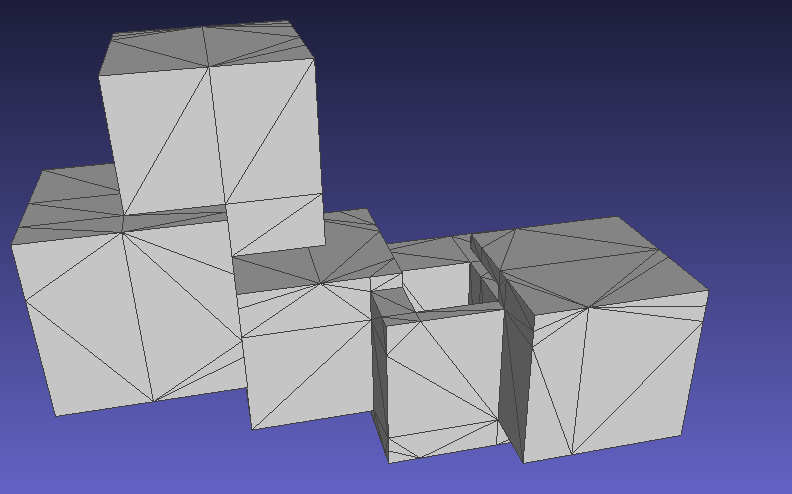
\includegraphics[width=\textwidth]{../image/5cubeoutcome.png}
          \caption{Worked}
        \end{minipage}
      \end{figure}
\end{frame}

\begin{frame}
    \begin{figure}
      \centering
      \begin{minipage}[b]{0.48\textwidth}
        \centering
        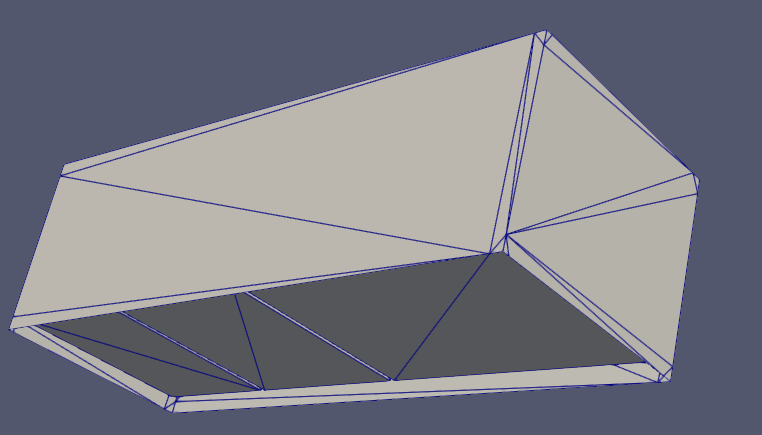
\includegraphics[width=\textwidth]{../image/3zonerefine.png}
        \caption{Refined Zones}
      \end{minipage}\hfill
      \begin{minipage}[b]{0.48\textwidth}
        \centering
        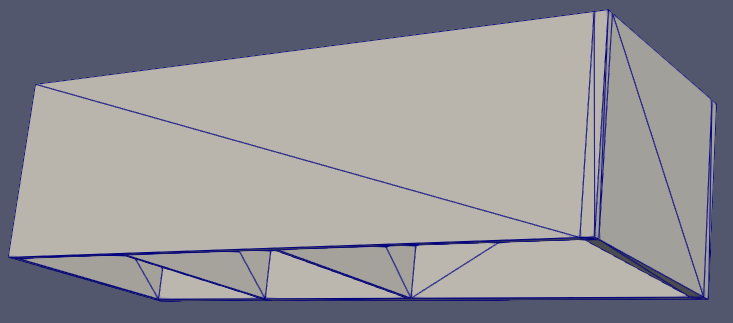
\includegraphics[width=\textwidth]{../image/3zones_not_refined.png}
        \caption{Not Refined Zones}
      \end{minipage}
    \end{figure}
\end{frame}

\begin{frame}{Comparison of Refined and Not Refined Zones}
    \begin{figure}
      \centering
      \begin{minipage}[b]{0.40\textwidth}
        \centering
        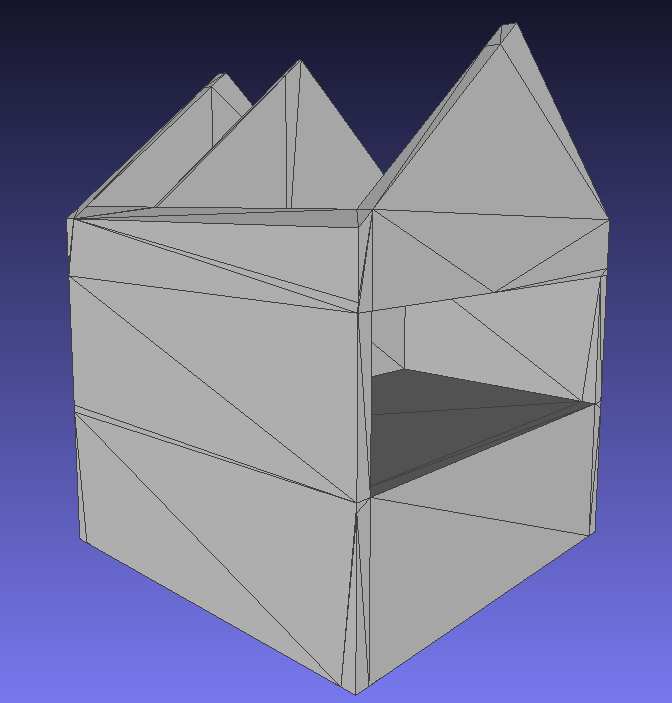
\includegraphics[width=\textwidth]{../image/ACJAsmin_refine.png}
        \caption{ACJAsmin Refined}
      \end{minipage}\hfill
      \begin{minipage}[b]{0.40\textwidth}
        \centering
        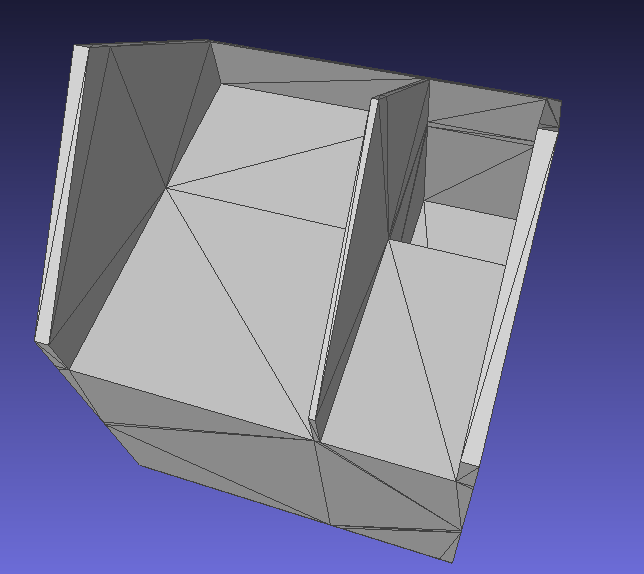
\includegraphics[width=\textwidth]{../image/Jasmin_hole.png}
        \caption{Jasmin Hole}
      \end{minipage}
    
    \end{figure}
\end{frame}

\begin{frame}
\begin{figure}
\begin{minipage}[b]{0.40\textwidth}
    \centering
    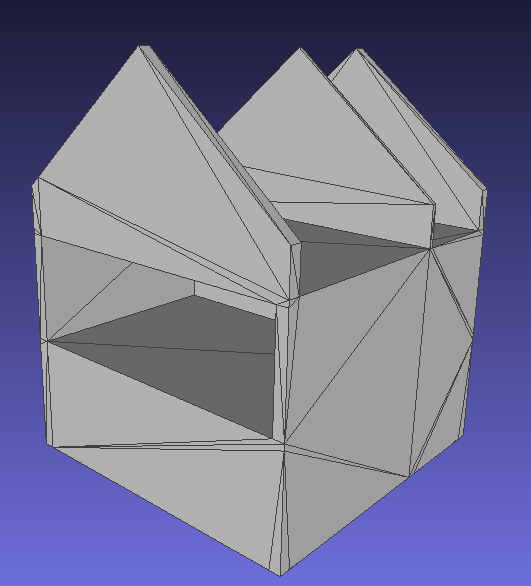
\includegraphics[width=\textwidth]{../image/ACJasmin_not_refined.png}
    \caption{ACJAsmin Not Refined}
  \end{minipage}\hfill
  \begin{minipage}[b]{0.40\textwidth}
    \centering
    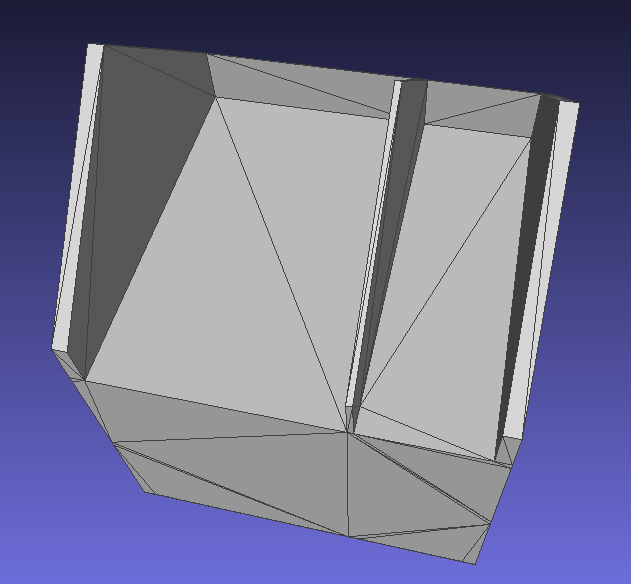
\includegraphics[width=\textwidth]{../image/Jasmin_not_refined_roof.png}
    \caption{Jasmin Not Refined Roof}
  \end{minipage}
\end{figure}

\end{frame}


\begin{frame}{Comparison of ACJASMIN Results}
    \begin{figure}
      \centering
      \begin{minipage}[b]{0.48\textwidth}
        \centering
        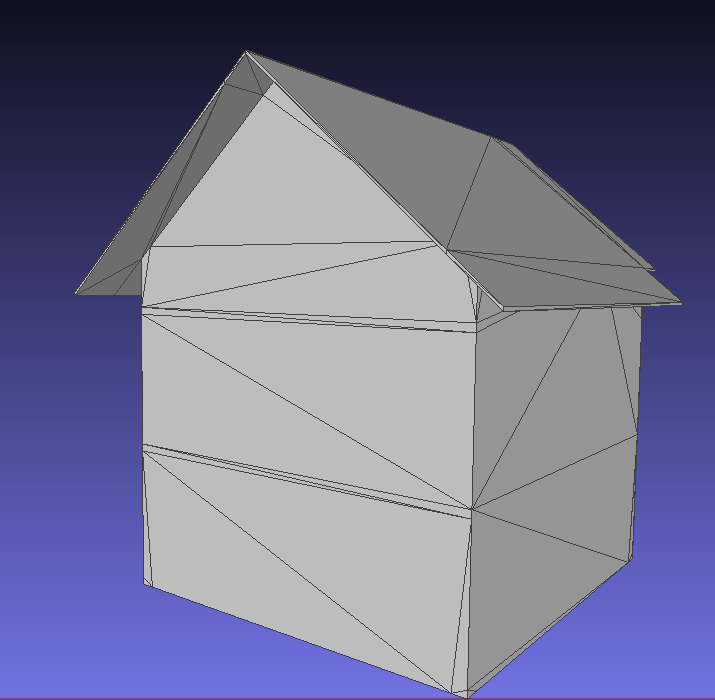
\includegraphics[width=\textwidth]{../image/ACJASMIN2000_0.04_refine.png}
        \caption{ACJASMIN Refined}
      \end{minipage}\hfill
      \begin{minipage}[b]{0.48\textwidth}
        \centering
        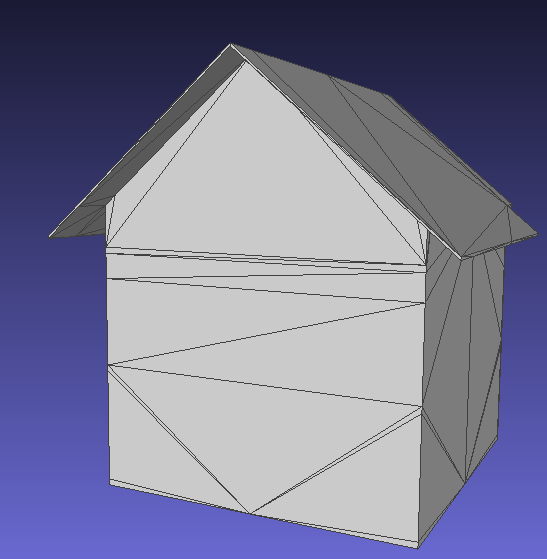
\includegraphics[width=\textwidth]{../image/ACJASMIN_2000_0.04.png}
        \caption{ACJASMIN Not Refined}
      \end{minipage}
    \end{figure}
    \end{frame}


\subsection{Performance}
\begin{frame}{Comparaison of performance}

    \begin{figure}
      \centering
      
      \begin{minipage}[b]{0.40\textwidth}
        \centering
        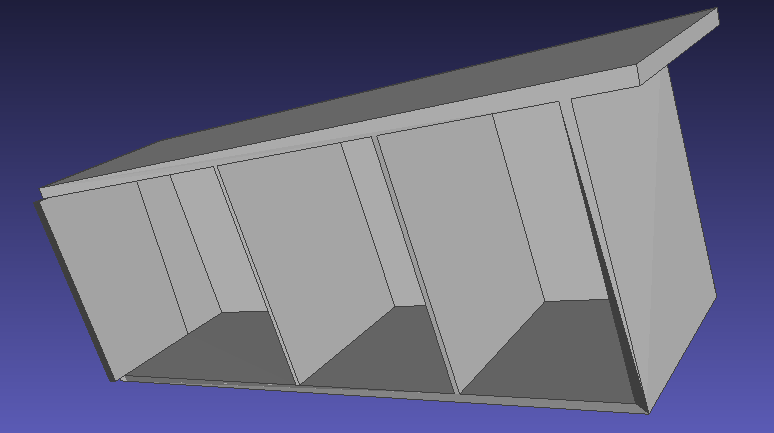
\includegraphics[width=\textwidth]{../image/tzones.png}
        \caption{Execution times 125s}
       
      \end{minipage}\hfill
      
      \begin{minipage}[b]{0.40\textwidth}
        \centering
        \includegraphics[width=\textwidth]{../image/3zones_final.png}
        \caption{Execution times 3s}
      \end{minipage}
    
    \end{figure}
    
    \end{frame}
\begin{frame}{Execution Time with Our Workflow on Three Zones}
    \begin{table}
        \centering
        \begin{tabular}{|l|c|c|c|c|}
          \hline
            Parameters & Default & mino=2000 & minp=500 & minp=100 \\
            \hline
            Shape detection & 7.97s & 8.18s & 5.76s & 1.62s \\
            \hline
            Kinetic space partition & 0.22s & 0.22s & 0.36s & 1.35s \\
            \hline
            Total execution & 8.2s & 8.41s & 6.13s & 2.98s \\
            \hline
        \end{tabular}
        \caption{Execution time with our workflow on Three Zones}
        \label{tab:execution_time}
    \end{table}
\end{frame}

\begin{frame}
  \begin{table}
    \centering
    \caption{Execution time on ACJasmin}
    \begin{tabular}{|l|c|c|c|c|}
      \hline
      default & minp=3000,dist=0.08 & minp=2000,dist=0.08 & minp=1200,dist=0.06 \\
      \hline
      407s & 58s & 39.8s & 31.5s \\
      \hline
      0.4s & 0.8s & 0.7s & 0.9s \\
      \hline
      407.5s & 58.8s & 40s & 32.5s \\
      \hline
    \end{tabular}
    \label{tab:execution_times}
    \end{table}
\end{frame}


\section{Conclusion}
\begin{frame}{Conclusion}
  \begin{itemize}
    \item From result overview: Better results and performance, but could not tried to apply FEM to the mesh.
    \item From personnal overwiew: earned how to code with an unknown package and the importance of team communication.
  \end{itemize}
\end{frame}

\section{Refereces}
\begin{frame}{references}
  \begin{thebibliography}{99}

    \bibitem{yu:hal-03767910}
    Yu, M., Lafarge, F., Oesau, S., \& Hilaire, B. (2022).
    \textit{Repairing geometric errors in 3D urban models with kinetic data structures}.
    \textit{ISPRS Journal of Photogrammetry and Remote Sensing, 192}, 1-12.
    \url{https://inria.hal.science/hal-03767910}
    
    \bibitem{bauchet:hal-02924409}
    Bauchet, J.-P., \& Lafarge, F. (2020).
    \textit{Kinetic Shape Reconstruction}.
    \textit{ACM Transactions on Graphics}.
    \url{https://inria.hal.science/hal-02924409}
    
    \bibitem{cgal:eb-24a}
    The CGAL Project. (2024).
    \textit{CGAL User and Reference Manual (5.6.1)}.
    CGAL Editorial Board.
    \url{https://doc.cgal.org/5.6.1/Manual/packages.html}
    
    \bibitem{yu:hal-03621896}
    Yu, M., \& Lafarge, F. (2022).
    \textit{Finding Good Configurations of Planar Primitives in Unorganized Point Clouds}.
    In \textit{CVPR 2022 - IEEE Conference on Computer Vision and Pattern Recognition}.
    \url{https://inria.hal.science/hal-03621896}
  \end{thebibliography}

\end{frame}

\begin{frame}
  \begin{thebibliography}{widestlabel}
    \bibitem{numpex2024}
Numpex. (2024).
\textit{Numpex Homepage}.
\url{https://numpex.org/}

\bibitem{cemosis2024}
Cemosis. (2024).
\textit{Cemosis Homepage}.
\url{https://www.cemosis.fr/}

\bibitem{hidalgo2024}
Hidalgo2. (2024).
\textit{Hidalgo2 Homepage}.
\url{https://www.hidalgo2.eu/}

\bibitem{ktirio2024}
Ktirio. (2024).
\textit{Ktirio Homepage}.
\url{https://ktirio.fr/}

\bibitem{titane2024}
Inria Titane Team. (2024).
\textit{Inria Titane Team Home Page}.
\url{https://team.inria.fr/titane/team/}

\end{thebibliography}
\end{frame}

\begin{frame}
  \begin{thebibliography}{widestlabel}
    \bibitem{cgal2024}
  CGAL. (2024).
  \textit{CGAL Homepage}.
  \url{https://www.cgal.org/}

  \bibitem{exam2024}
Numpex. (2024).
\textit{Numpex Exa-MA methods and algorithms for exascale}.
\url{https://numpex.org/exama-methods-and-algorithms-for-exascale/}

\bibitem{cgalksr2024}
CGAL. (2024).
\textit{User Manual for KSR}.
\url{https://cgal.geometryfactory.com/CGAL/doc/master/Kinetic_surface_reconstruction/index.html}

\bibitem{feelpp2024}
Feel++ Project. (2024).
\textit{User Manual Feel++ Toolboxes}.
\url{https://docs.feelpp.org/toolboxes/latest/index.html}

\end{thebibliography}

\end{frame}

\end{document}
